\chapter{Service Instructions for Vise SEL 36 For Use on Universal Milling Machine 13 \small{Accessory No. 36}}

\section*{Main Features}

\begin{tabular}{@{}ll@{}}
    Jaw Width       & 85 mm         \\
    Maximum Opening & 60 mm         \\
    Jaw Height      & 37 mm         \\
    Swiveling       & \(360^\circ\) \\
    Inclination     & \(360^\circ\) \\
    Stop every      & \(15^\circ\)  \\
\end{tabular}

\section*{Cleaning, Lubrication, and Maintenance}

Upon receipt and during operation, follow the provided instructions for the machine, which are valid and must be observed.
The vise includes an oiler for lubrication using a pump.
The horizontal position at \(0^\circ\) (closed jaws) allows lubrication of the sliding jaw and the screw; the vertical position at \(90^\circ\) (jaws on the oiler side) allows lubrication of the guide.

\section*{Usage}

The base is fixed on one of the T-slots of the table using two rods. Two locator blocks ensure alignment.

The vise is locked in all positions in the horizontal plane by two rods.
Inclination can be done throughout the circumference, degree by degree.
However, the exact position is ensured every \(15^\circ\) by a hardened piston.
Locking is done using a keyed nut delivered with the vise.

Good milling results are obtained by following the procedure indicated in the sketch below:

\begin{figure}[h]
    \centering
    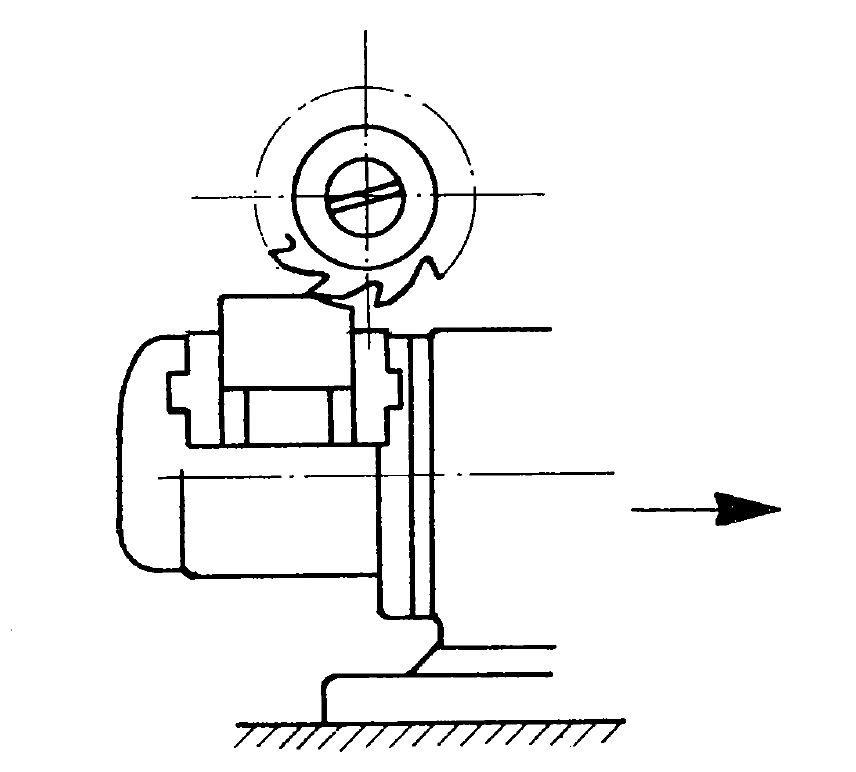
\includegraphics[width=0.5\linewidth]{images/page_43}
    \caption{Milling direction}
    \label{fig:milling_direction}
\end{figure}
